\section{Изучение эталонных кристаллов Si и Ge}

Для измерения ПЭЯ Si, с учетом ранее обозначенных приборных ограничений, наиболее подходят три семейства кристаллографических плоскостей \hkl{11 3 1}, \hkl{9 7 1} и \hkl{9 5 5} c $2\theta = 96.737\degree$.
В случае Ge выбраны семейства \hkl{10 6 0} и \hkl{8 6 6} с $2\theta = 93.949\degree$.
Поиск подходящих рефлексов средствами программы APEX3 можно сделать только в ручном режиме, т.е. последовательно прелагая значения \hkl(h k l).
Возможны два варианта расчетов: первый предполагает определение углов для вывода кристаллографического направления навстречу пучку ($\varphi_0$ и $\omega_0$), второй --- углов для установки кристаллографической плоскости в отражающее положение при положении детектора в отрицательных углах $2\theta_D$.
В обоих вариантах предлагается только одно значение $\varphi$ (из двух возможных).
Такого функционала совершенно недостаточно для учета эксцентриситета образца: согласно~\cite{Ponomarev:1969} необходимо подобрать пару рефлексов \hkl(h k l), которые можно зафиксировать при положениях гониостата $\omega \approx \pm 90\degree$ (см. рис.~\ref{fig:eccentr}).
В случае Si, число симметрично связанных плоскостей равно 120 (для Ge –-- 48) и сделать это средствами программы APEX3 проблематично.
Необходимые расчеты были проведены по программе James.

\begin{figure}[ht!]
    \centering
    \begin{subfigure}{0.5\textwidth}
    \centering
    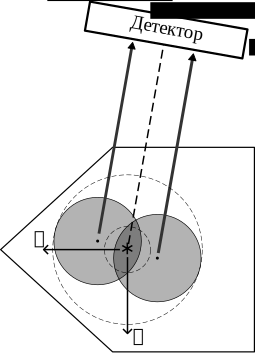
\includegraphics[]{eccentr.pdf}
    \caption{}%
    \label{fig:eccentr_neg}
    \end{subfigure}%
    \begin{subfigure}{0.5\textwidth}
    \centering
    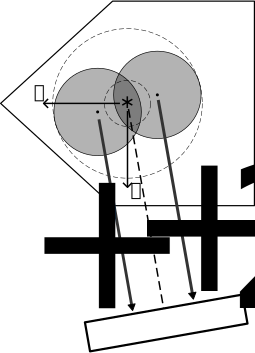
\includegraphics[]{eccentr_2.pdf}
    \caption{}%
    \label{fig:eccentr_pos}
    \end{subfigure}
    \caption{
        Схемы эксперимента для учета эксцентриситета образца, связанного с поворотом вокруг оси $\omega$ (ось $\omega$ идет перпендикулярно плоскости чертежа, выход показан звездочкой).
        a --- показаны два положения образца (условные центры обозначены жирными точками), при которых проводятся съемки рефлексов и определяются положения максимумов – $X_1$ и $X_2$.
        Окружность меньшего диаметра соответствует сфере сведения, большая окружность (выделена пунктиром) ограничивает область расположения образца.
        Показана система координат: направление $x$ проходит через ось $\omega$ в направлении первичного пучка (условно показано, что в общем случае $x$ не совпадает с максимумом первичного пучка);
        $y$ --- направление перпендикулярное $x$ и лежащее в экваториальной плоскости.
        Направление $z$ совпадает с осью $\omega$.
        b --- схема для симметричного положения детектора.
    }%
    \label{fig:eccentr}
\end{figure}

Первая часть программы James позволяет находить среди множества плоскостей, связанных симметрией такие, которые можно вывести в отражающее положение хотя бы при одном (из двух симметричных) положении детектора.
Для этого используется информация о текущей ориентации кристалла на гониометре, т.е. p4p-файл, в котором находится матрица ориентации UB~\cite{Busing:1967} и предварительные значения ПЭЯ.
Углы гониометра $\varphi$ и $\omega$, необходимые для выведения каждой плоскости в отражающее положение на экваториальную плоскость, вычисляются исходя из известной длины волны, размеров пикселя, расстояния до детектора и других неизменных параметров прибора.
В каждом случае проверяются геометрические ограничения прибора.
Полученная информация для всех подходящих рефлексов собирается в таблицу Excel, ее можно проанализировать и провести отбор.

Вторая часть программы James связана с обработкой полученных фреймов, т.е. описанием 2D-профиля дублета. На входе она использует p4p-файл и информацию о примерном положении центра детектора (результат юстировки, прямое определение, калибровка).
Из экспериментального фрейма вырезается центральная область ($X = \pm 30\unit{пикс.}$, $Y = \pm 15\unit{пикс.}$), в которой, исходя из $2\theta_D \approx 2\theta_{hkl}$, должен находиться искомый рефлекс.
Медианное значение интенсивности принимается за начальное значение фона.
Пиксели с интенсивностью больше заранее заданной принимаются за ''горячие пиксели'' и их значения приравниваются среднему значению по 8 соседним пикселям.
После учета горячих пикселей максимум интенсивности в выбранной области назначается примерным положением $K\alpha_1$-составляющей.
Далее, исходя из значений $D$ и $2\theta$ рассчитывается положение $K\alpha_2$-составляющей и обе точки смещаются так, чтобы теоретическое положение $K\alpha_1$ совпадало с координатами найденного максимума интенсивности.
Аппроксимация дублета проводится двумя независимыми  функциями 2D-Gauss, т.е. без закрепления междублетного расстояния и соотношения интенсивностей составляющих $2/1$.
Направлениями главных осей берутся вдоль координат детектора $X$ и $Y$ детектора.
В наших экспериментах именно функция 2D-Gauss наиболее хорошо описывала форму пика при минимальном числе уточняемых параметров: координаты максимума, полуширины (ширина на половине высоты, FWHM) в направлениях $X$ и $Y$, и интегральная интенсивность.

\subsection{Оценка и учет эксцентриситета образца Si}

Несмотря на тщательную центрировку образца (в том числе с контрольными разворотами по оси $\omega$) крайне сложно точно определить центр образца, особенно при его неопределенной форме.
Можно ожидать, что при повороте вокруг оси $\omega$ центр образца движется по окружности, а сам образец описывает торообразную поверхность, ее условный внешний контур показан на рис.~\ref{fig:eccentr} штриховой окружностью.
Выход оси $\omega$ показан звездочкой: считаем, что в общем случае ось не пересекается центром первичного пучка.
Подобную картину можно ожидать и при повороте образца вокруг оси $\varphi$.
Так как для использованного гониометра паспортное значение диаметра сферы сведения осей (sphere of confusion) составляет 7~мкм, центр образца при повороте вокруг обеих осей движется по достаточно сложной траектории.

Для оценки смещений центра образца при повороте вокруг оси $\varphi$, среди доступных для измерения рефлексов от семейств кристаллографических плоскостей типа \hkl{11 3 1}, \hkl{9 7 1} и \hkl{9 5 5}, было выбрано 10 вариантов, у которых значения $\omega$ лежат в интервале от $-82\degree$ до $-95\degree$.
Это примерно соответствует позиции образца при центрировании.
Все съемки проведены при положении детектора: $2\theta_D = -96.7\degree$, $D = 128.53\unit{мм}$.
Зависимость $X(\varphi)$ представлена на рис.~\ref{fig:eccentrSi}а.
Интервал значений $X$ составляет $\approx 0.3$~пикселя, что с учетом размера пикселя, соответствует смещениям центра образца с оси $\varphi$ на 20~мкм.

\begin{figure}[ht!]
    \centering
    \includegraphics[width=0.8\textwidth]{eccentrSi.png}
    \caption{
        Смещение максимумов дифракционных отражений Si \hkl(11 3 1), \hkl(9 7 1) и \hkl(9 5 5) по оси $X$ детектора из-за эксцентриситета образца: a --- зависимость координаты $X$ от угла $\varphi$ (значения углов $\omega \approx 270\degree$);
        b --- зависимость координаты $X$ от угла $\omega$ (значения углов $\varphi$ лежат в интервале $\range{283.6}{300.7}\degree$)
    }%
    \label{fig:eccentrSi}
\end{figure}

Таким образом, два проведенных эксперимента показали одинаковые картины эксцентриситетов, связанных с поворотами образца вокруг осей $\omega$ и $\varphi$.
При измерении ПЭЯ наиболее разумно исключить влияние именно последнего, тогда далее можно использовать подход, предложенный в~\cite{Ponomarev:1969}.
Он заключается в съемке фриделевской пары со значениями $\omega \approx \pm 90\degree$, что соответствует крайним положениям центра образца в направлении первичного пучка.
На рис.~\ref{fig:eccentr} центры образцов показаны жирными точками.
Очевидно, что при таких положениях образца можно ожидать максимальных смещений дифракционных рефлексов.
Среди всех вариантов, предложенных программой James, были выделены 5 фриделевских пар, удовлетворяющих этому критерию.
Их индексы и установочные углы $\varphi$ и $\omega$ представлены в табл.~\ref{tab:Si} Приложения.
Там же даны координаты максимумов рефлексов, зарегистрированных при симметричных положениях детектора $2\theta_D = 96.7\degree$ и средние значения для каждой пары $\left<X\right> = (X_1 + X_2) / 2$.
Как следует из рис.~\ref{fig:eccentr} значения $\left<X\right>$ соответствует мнимому положению кристалла на оси вращения $\omega$.
Для учета эксцентриситета в формуле~(\ref{eq:bond2}) вместо значений $X$ необходимо использовать значения $\left<X\right>$.
Чтобы различать рефлексы, зарегистрированные при симметричных положениях детектора, введем надстрочные индексы <<$-$>> и <<$+$>>, тогда выражение~\ref{eq:bond2} можно представить в следующем виде:
\begin{equation}\label{eq:bond4}
    2\theta_{hkl} = 2\theta_D + \gamma (\tensor*[^-]{X}{_1} + \tensor*[^-]{X}{_2} - \tensor*[^+]{X}{_1} - \tensor*[^+]{X}{_2}) / 4 = 2\theta_D + \gamma (\left<\tensor*[^-]{X}{}\right> - \left<\tensor*[^+]{X}{}\right>) / 2
\end{equation}
где $\gamma$ --- угловой размер пикселя.

\subsection{Определение угловых размеров пикселя}

При регистрации рефлекса центральной областью детектора (как в нашем случае) значение $\gamma$ можно вычислить исходя из физических размеров пикселя $P$ (в нашем случае 0.1353~мм) и расстояния от образца до детектора $D$ (в нашем случае 128.53~мм) по формуле:
\begin{equation}\label{eq:pixsize}
    \gamma = \frac{P}{D}
\end{equation}
Однако значение $D$, которое показывает прибор, всегда можно поставить под сомнение.
Правильнее провести калибровку положения детектора, например, согласно методике~\cite{Panchenko:2023}.
Для этого съемка эталонного монокристалла Si была проведена путем $\omega$-сканирования интервалов $10\degree$ в области углов $200\degree$ при пяти положениях кристалла по углу $\varphi$ (шаг $10\degree$).
Обработка полученных фреймов проведена по программе SearchXY~\cite{Panchenko:2023}.
В результате получено значение $D = 128.21\unit{мм}$.
Развороты детектора (rot1, rot2, rot3) в наших экспериментах можно не учитывать, т.к. регистрация рефлексов проводится центральной областью детектора.
Итоговое значение $\gamma = 0.06033\degree$.

Не всегда проведение полной калибровки положения детектора целесообразно, т.к. она занимает достаточно много времени.
Можно согласно~\cite{Gromilov:2022} использовать данные о положении $K\alpha_1$- и $K\alpha_2$-составляющих любого из изученных рефлексов эталона, тогда по разнице значений $X$ и теоретическим положениям углов $2\theta$  $K\alpha_{1,2}$-составляющих значение $\gamma$ вычисляют по формуле:
\begin{equation}\label{eq:pixsize_exp}
    \gamma = \frac{2\theta_2 - 2\theta_1}{\Delta X}
\end{equation}

Другой подход к определению $\gamma$ основан на съемке одного и того же рефлекса при двух угловых положениях детектора.
Так, рефлекс \hkl(-11 1 -3) Si был отснят при $2\theta_A = 96.4\degree$ и $2\theta_B = 97.0\degree$.
Смещение максимума $\Delta X$ позволяет провести вычисление $\gamma$ по формуле:
\begin{equation}\label{eq:pixsize_exp_2}
    \gamma = \frac{2\theta_A - 2\theta_B}{\Delta X} = 0.06033\degree
\end{equation}

Отметим, что такой подход позволяет проводить измерения при минимальных отклонениях рефлекса от центра детектора.
Полученное значение идеально совпадает с результатом, полученным по результатам полной калибровки.

\subsection{Вычисление ПЭЯ Si}

Полученное значение $\gamma$ позволяет вычислить $a_\text{Si}$.
При произвольном выборе рефлексов из табл.~\ref{tab:Si} Приложения расчет согласно~\ref{eq:bond2} приводит к значениям угла $2\theta$ в интервале $\range{96.722}{96.747}\degree$: отклонения от теоретического значения $96.734\degree$ достигают $0.013\degree$.
Учет эксцентриситета согласно~\ref{eq:bond4} с использованием произвольных пар средних значений $\left<\tensor*[^-]{X}{}\right>$ и $\left<\tensor*[^+]{X}{}\right>$ уменьшает интервал значений $2\theta$ до $\range{96.730}{96.736}\degree$ а отклонения от теоретического значения не превышают $0.004\degree$.
Использование рефлексов с близкими значениями углов $\varphi = -66.31\degree$ и $59.35\degree$ (индексы рефлексов выделены в табл.~\ref{tab:Si} Приложения жирным) позволяет учесть эксцентриситет, связанный с поворотом образца вокруг оси $\varphi$.
Конечные результаты уточнения: $2\theta = 96.732\degree$, $d = 0.47452 (3)\unit{\AA}$, $\Delta d / d = 6.2 \cdot 10^{-5}$, $a = 5.4311(3)\unit{\AA}$ (в скобках указаны абсолютные погрешности, вычисленные для $\Delta 2 \theta = 0.004\degree$).
Можно отметить, что полученное значение $a_\text{Si}$ отклоняется от эталонного всего на $0.00006\unit{\AA}$.
Чтобы полностью исключить влияние эксцентриситета, связанного с поворотом кристалла вокруг оси $\varphi$, необходимо вывести одно из кристаллографических направлений вдоль оси $\omega$, тогда измерения можно проводить на рефлексах типа \hkl{h k 0}.
При использовании гониометра с изменяемым углом $\chi$ (т.е. четырехкружного) такая проблема не возникает.
В нашем случае угол $\chi$ на гониометре фиксирован, а штатные гониометрические головки предполагают только линейные перемещения образца.

\subsection{Вычисление ПЭЯ Ge}

Для устранения эксцентриситета, связанного с поворотом кристалла вокруг оси $\varphi$ монокристалл Ge был смонтирован на оригинальной гониометрической головке, имеющей возможность поворота образца вокруг одной оси на $\pm 10\degree$ (далее гониометрическая $\chi$-головка).
После определения ориентации кристалла, с помощью программы James были рассчитаны углы для выведения кристаллографического направления вдоль оси $\omega$, для этого был использован следующий алгоритм.

Повороты образца описываются эйлеровыми углами $\varphi$, $\omega$ и $\chi$.
Правосторонняя декартова система координат гониометра задана следующим образом.
Направление оси $x$ совпадает с направлением первичного пучка.
Если смотреть навстречу $x$, то положительным изменением угла $\omega$ будет вращение против часовой стрелки.
Ось $z$ выбирается в направлении оси $\omega$ и против направления оси $\varphi$ (в нулевом положении для четырехкружного гониометра).
Направление оси $y$ задается автоматически.
Ось $\chi$ направлена против оси $x$, в нашем случае соответствующий ей угол поворота фиксирован и равен приблизительно $55\degree$.

Нулевой угол дуги нашей гониометрической головки обозначим $\chi^\ast$.
Т.к. кристаллографическое направление можно вывести вдоль или против $z$, то число возможных вариантов $\chi$ и $\chi^\ast$ может быть равно 4 (2 в вырожденном случае) или 0 (если процедура невозможна).
Ограничение значений угла $\chi^\ast$ связано с диапазоном углов дуги гониометрической головки, в нашем случае $\pm 10\degree$.

Если задать кристаллографическое направление \hkl[h k l] в виде трехмерного вектора $s$, получающегося домножением вектора-столбца \hkl(h k l) на матрицу ориентации UB, то определить возможность выведения рефлекса можно по углу $\theta_s$ между $s$ и $x$ и полярному углу $\varphi$ проекции $s$ на плоскость $yz$ (рис.~\ref{fig:scheme}).
Кристаллографическое направление можно вывести вдоль оси $\omega$ если $\sin{\theta_s} > \cos{\chi}$.
В этом случае углы $\chi^\ast$ будут равны:
\[ \varphi_s - \arcsin\left(\frac{\cos{\chi}}{\sin{\theta_s}}\right) \]
\[ \varphi_s + \arcsin\left(\frac{\cos{\chi}}{\sin{\theta_s}}\right) + 180\degree \]
\[ \varphi_s + \arcsin\left(\frac{\cos{\chi}}{\sin{\theta_s}}\right) \]
\[ \varphi_s - \arcsin\left(\frac{\cos{\chi}}{\sin{\theta_s}}\right) + 180\degree \]

При значении $\cos{\chi} > 0$ первые два угла соответствуют выведению $s$ вдоль $x$, а другие --- $-x$. При смене знака $\cos{\chi}$ картина меняется на противоположную.
Соответствующие углы $\omega$ будут равны:
\[\arctan\left(-\sqrt{\sin^2{\theta_s} - \cos^2{\chi}}, -\cos{\theta_s}\right)\]
\[\arctan\left(\sqrt{\sin^2{\theta_s} - \cos^2{\chi}}, -\cos{\theta_s}\right)\]
\[\arctan\left(\sqrt{\sin^2{\theta_s} - \cos^2{\chi}}, \cos{\theta_s}\right)\]
\[\arctan\left(-\sqrt{\sin^2{\theta_s} - \cos^2{\chi}}, \cos{\theta_s}\right)\]

где $\arctan(y, x)$ –-- полярный угол точки с координатами $(x, y)$ на координатной плоскости. 

\begin{figure}[ht!]
    \centering
    
\includegraphics{scheme.pdf}
    \caption{
        Схема направления осей гониометра ($\varphi$, $\chi$, $\omega$) и дополнительного поворота монокристалла на гониометрической головке ($\chi^\ast$) в проекции $yz$.
        Экваториальная плоскость гониометра показана пунктирной линией.
        Вектор кристаллографического направления $s$ показан стрелкой.
        Путь поворота вектора по трем углам $\chi^\ast$, $\varphi$, $\chi$ обозначен жирной ломаной линией.
        Точки 1--4 обозначают 4 возможные положения, через которые кристаллографическое направление может быть выведено вдоль или навстречу оси $\omega$.
    }%
    \label{fig:scheme}
\end{figure}

Расчеты для монокристалла Ge показали, что вдоль оси $\omega$ можно вывести направление \hkl{0 1 0}, т.к. для него значение угла $\chi^\ast = 2.2\degree$.
После соответствующего поворота образца на гониометрической $\chi$-головке, исследование в схеме Бонда было проведено по рефлексам типа \hkl{10 0 6} (теоретическое значение $2\theta = 93.943\degree$).
Все рефлексы регистрировали при одинаковых значениях угла $\varphi = -179.06\degree$.
Приборные ограничения позволили отснять только 12 из 16 теоретически возможных рефлексов, координаты их максимумов приведены в табл.~\ref{tab:Ge} Приложения.
При произвольных сочетаниях рефлексов, возможны 36 вариантов пар, тогда значения $2\theta$, вычисленные согласно~\ref{eq:bond2}, лежат в интервале $\range{93.935}{93.958}\degree$.
Максимальные отклонения от теоретического значения достигают $0.015\degree$.
Для учета эксцентриситета согласно~\ref{eq:bond4} были использованы 4 пары значений $\left<X\right>$, при этом вычисленные значения $2\theta$ укладываются в узкий интервал $\range{93.943}{93.945}\degree$, а отклонения от теоретического значения не превышают $0.001\degree$.
Если использовать среднее значение $2\theta = 93.945\degree$, то: $d = 0.48515 (3)\unit{\AA}$, $\Delta d / d = 6.5 \cdot 10^{-5}$, $a = 5.6578 (4)\unit{\AA}$.
Отклонение полученного $a_\text{Ge}$ от теоретического значения $5.657885\unit{\AA}$ составляет 
$0.0001\unit{\AA}$.

Анализ координат $Y$ рефлексов Ge (см. табл.~\ref{tab:Ge} Приложения) позволяет оценить точность выведения направления $b$ вдоль оси $\omega$.
Для этого можно построить зависимости $Y$ от $\omega$ для экспериментов, проведенных при двух симметричных положениях детектора $2\theta_D = 93.9\degree$.
В обоих случаях зависимости хорошо описываются синусоидами, но при $2\theta_D = -93.9\degree$ фаза сдвигается на $\theta$, а при $2\theta_D = +93.9\degree$ на $\theta + 180\degree$.
Для одновременной обработки всех рефлексов значения сдвигов вычитали из первичных значений $\omega$.
Из построенной аппроксимации (см. рис.~\ref{fig:eccentrGe}) следует, что максимальная разница значений $Y$ составляет $\approx 2.2\unit{пикс.}$, что соответствует отклонению направления $b$ от оси $\omega$ $0.13\degree$.
Такой показатель соответствует цене нониусной шкале дуги использованной гониометрической головки.
Т.к. отклонение лежит в плоскости дуги гониометрической головки, можно утверждать, что оно связано преимущественно именно с погрешностью установки угла $\chi^\ast$, а не угла $\varphi$.

\begin{figure}[ht!]
    \centering
    \includegraphics[height=0.5\textwidth]{eccentrGe.png}
    \caption{
        Зависимость координат $Y$ от угла $\omega$ для монокристалла Ge.
        Точки полученные при положении детектора $2\theta_D = -93.9\degree$ обозначены кружками, а при $2\theta_D = +93.9\degree$ --- квадратами.
        Аппроксимация всех точек проведена с помощью МНК, использована функция $Y = a_0 + a_1 \cos(\omega - \omega_1)$
    }%
    \label{fig:eccentrGe}
\end{figure}

Выведение кристаллографического направления вдоль оси $\omega$ позволяет не только определять межплоскостные расстояния и ПЭЯ, но и углы между кристаллографическими плоскостями типа \hkl[h 0 l].
Так, для изученного монокристалла Ge было проведено измерение угла между плоскостями \hkl[6 0 -10] и \hkl[10 0 -6].
Для этого получена зависимость интенсивности рефлекса от угла $\omega$ с помощью $\omega$-сканирования диапазона $0.4\degree$, содержащего максимум интенсивности рефлекса от $K\alpha_1$ с шагом $0.002\degree$.
Для каждой позиции проводили суммирование интенсивности всех пикселей в прямоугольной области детектора $50\times30$.
Значение угла $\omega$, при котором достигается максимальная интенсивность, было получено аппроксимацией полученной зависимости $I(\omega)$ полиномом второй степени.
В результате, полученные значения углов $\omega$ составили $67.6113 (2)\degree$ и $95.6731 (2)\degree$ для рефлексов \hkl[6 0 -10] и \hkl[10 0 -6] соответственно.
Разница значений составила $28.0618 (4)\degree$, что отличается от идеального значения $28.0725\degree$ на $0.0107 (4)\degree$.

Проведенные эксперименты с эталонными монокристаллами показывают, что учет эксцентриситета образца вокруг оси $\omega$ с ограничением углов $\varphi$ позволяет получать значения углов $2\theta$ с точностью не хуже $0.004\degree$.
Особо отметим, что это не среднее значение по нескольким экспериментам, а максимальное отклонение.
При сохранении такого показателя повышение точности измерений ПЭЯ возможно лишь при увеличении углов $2\theta$.
При использовании дифрактометра, оборудованного 2D-детектором, это можно достичь лишь путем использования рефлексов на краю детектора.
Так, при установке детектора в позиции $D = 128.5\unit{мм}$ и $2\theta_D = 97\degree$ можно регистрировать рефлексы вплоть до $118\degree$, что теоретически должно привести к уменьшению относительной ошибки $\Delta d / d$ вдвое.
Однако, такой путь предполагает проведение двух полных калибровок прибора при симметричных положениях детектора.Гораздо перспективней использовать дополнительный детектор меньших размеров, как это будет описано далее.

Другое ограничение точности измерений связано с большой шириной дифракционных отражений: даже для исследованных эталонных монокристаллов значения FWHM достигают $0.12\degree$, что в первую очередь обусловлено расходимостью первичного пучка.
К недостаткам лабораторных дифрактометров можно отнести и недостаточную светосилу.
В нашем случае, несмотря на использование микрофокусного источника 3-го поколения, измерение одного рефлекса Si составило 2 часа, т.е. съемка 4-х рефлексов для учета эксцентриситета занимала 8 час.
Большое время эксперимента существенно ограничивает эксперименты по изучению динамики изменения ПЭЯ при внешних воздействиях.
Конечно, можно пожертвовать точностью и перейти к исследованию рефлексов с меньшими значениями $2\theta_D$, но большей интенсивностью.
Все указанные недостатки могут быть существенно уменьшены при переходе на синхротронное излучение.
Так на станции 1.2 «Структурная диагностика» ЦКП СКИФ (г. Новосибирск) будет установлен монокристальный дифрактометр.
Даже если он будет оснащен двухкружным гониометром, минимальная дооснастка (гониометрическая $\chi$-головка, дополнительный детектор) позволит проводить прецизионное измерение ПЭЯ с $\Delta d / d \approx 10^{-6}$.
Однако, для измерения параметров элементарной ячейки кристаллов с низкой симметрией (триклинной или моноклинной) предпочтительней использовать четырехкружный гониометр, что позволит избежать нескольких переклеек кристалла.
